\documentclass{article}

\setlength{\parskip}{0.4\baselineskip}
\setlength{\parindent}{0in}

\usepackage[square,numbers]{natbib}
\bibliographystyle{abbrvnat}

\usepackage[utf8]{inputenc}
\usepackage{amssymb}
\usepackage{amsthm}
\usepackage{amsmath}
\usepackage{amsfonts}
\usepackage{mathtools}

\usepackage{microtype}
\usepackage{float}
\usepackage{hyperref}
\hypersetup
{
	colorlinks,
	linkcolor = blue,
	citecolor = blue,
	urlcolor = blue,
	filecolor = blue,
	breaklinks,
}

\usepackage{color}
\usepackage{graphicx}
\graphicspath{ {images/} }

\usepackage{algpseudocode}
\usepackage{algorithm}
\MakeRobust{\Call}

\usepackage[accepted]{icml2018}


\newtheorem{lemma}{Lemma}[section]
\newtheorem*{example}{Example}
\newtheorem{thm}{Theorem}[section]
\newtheorem{corollary}{Corollary}[thm]
\theoremstyle{definition}
\newtheorem{definition}{Definition}[section]
\theoremstyle{remark}
\newtheorem*{remark}{Remark}

\DeclareMathOperator{\Hom}{Hom}
\DeclareMathOperator{\Ext}{Ext}
\DeclareMathOperator{\coker}{coker}
\DeclareMathOperator{\im}{im}
\DeclareMathOperator{\st}{st}
\DeclareMathOperator{\lk}{lk}
\DeclareMathOperator{\degr}{deg}

\newcommand{\reducedhom}{\tilde{H}}
\newcommand*\cl[1]{\overline{#1}}
\newcommand{\catname}[1]{{\normalfont\textbf{#1}}}
\newcommand{\bigslant}[2]{{\raisebox{.2em}{$#1$}\left/\raisebox{-.2em}{$#2$}\right.}}
\newcommand{\vr}[2]{{\text{VR}_{#1}(#2)}}
\newcommand{\cech}[2]{{\check{C}_{#1}(#2)}}
\newcommand{\strat}[1]{{\text{Strat}(#1)}}
\newcommand{\transpose}[1]{#1^\top}
\newcommand{\norm}[1]{\left\lVert#1\right\rVert}
\newcommand{\wordv}[1]{v_\text{#1}}
\DeclarePairedDelimiterX\setc[2]{\{}{\}}{\,#1 \;\delimsize\vert\; #2\,}
\newcommand\restr[2]{{% we make the whole thing an ordinary symbol
		\left.\kern-\nulldelimiterspace % automatically resize the bar with \right
		#1 % the function
		\vphantom{\big|} % pretend it's a little taller at normal size
		\right|_{#2} % this is the delimiter
}}
\newcommand{\zmod}[1]{\mathbb{Z}/#1\mathbb{Z}}

\icmltitlerunning{Report Template}

%custom settings:
\usepackage{todonotes}
%\listoftodos

\begin{document}

\twocolumn[
\icmltitle{Report Template}

\icmlsetsymbol{equal}{*}

\begin{icmlauthorlist}
\icmlauthor{Student One}{keio}
\icmlauthor{Student Two}{waseda}
\end{icmlauthorlist}

\icmlaffiliation{keio}{Keio University, Department of Economics}
\icmlaffiliation{waseda}{Waseda University, Department of Mathematics}
\icmlcorrespondingauthor{Student One}{studentone@keio.jp}
\icmlkeywords{artificial intelligence, neural networks, deep learning}
\vskip 0.3in
]

\printAffiliationsAndNotice{\icmlEqualContribution}




%----------------------------------------------------------------------------------------
%	ABSTRACT, KEYWORDS AND ABBREVIATIONS
%----------------------------------------------------------------------------------------

\begin{abstract}
   Summarize your assignment and results briefly here... 
\end{abstract}

%------------------------------------------------



\section{Introduction}

Add more sections below, cite some papers like so \cite{vaswani2017attention}, and include some diagrams like so \ref{transformer}.

\begin{figure}[!h]
	\centering
	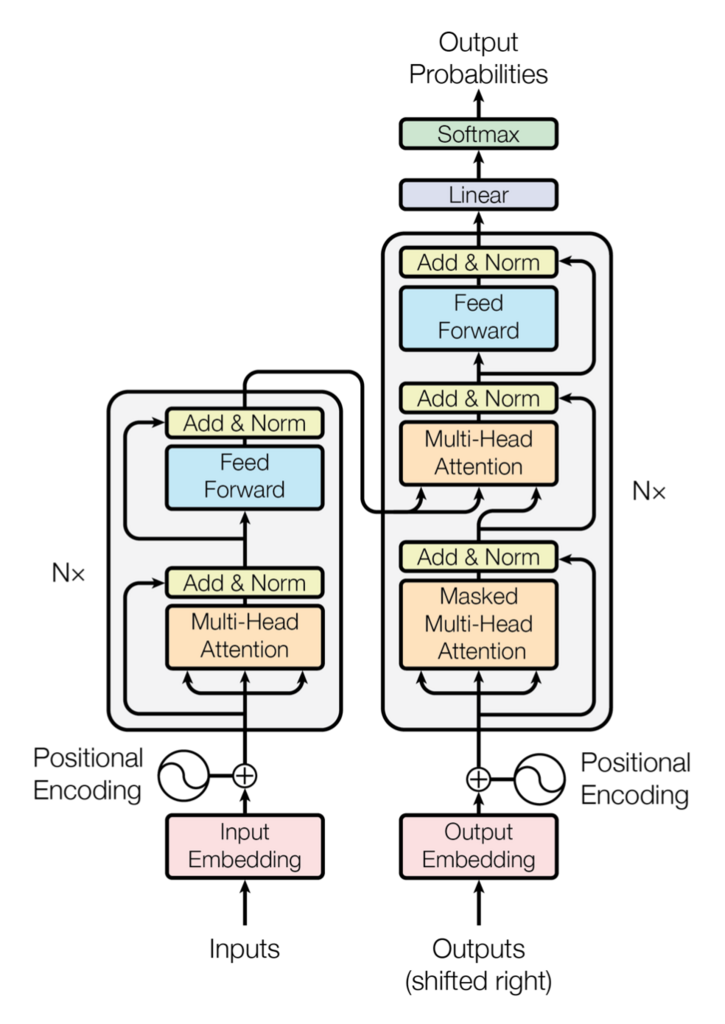
\includegraphics[width=0.49\textwidth]{img/transformer.png}
	\caption{Transformer diagram.}
	\label{transformer}
\end{figure}

\begin{itemize}
	\item include sections for each part of the assignment
    \item describe your model and implementation
    \item answer questions for each part
\end{itemize}

\bibliography{main}

\end{document}
